\clearpage\section{Architecture}

My project is not just a language and a compiler for it, but rather a much larger ecosystem. It needs to store, compile, and run scripts. To achieve this, I designed a multi-component architecture depicted in figure \ref{fig:comp_arch}.

\begin{figure}[h]
    \centering
    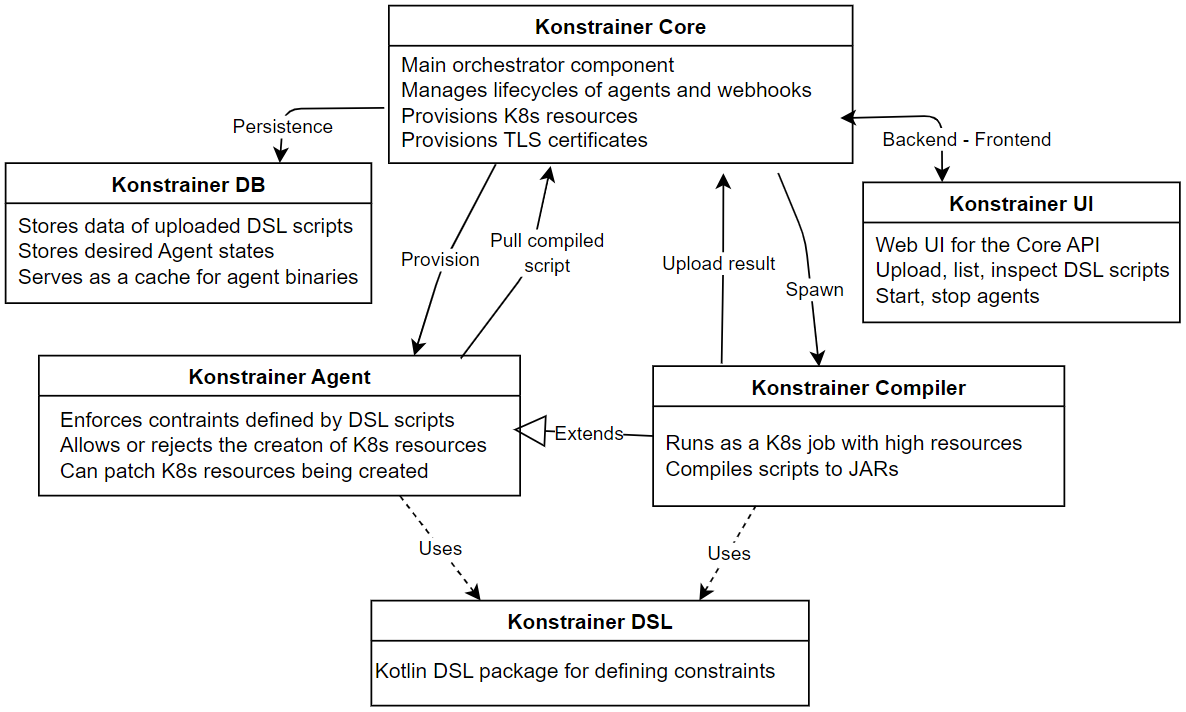
\includegraphics[width=130mm, keepaspectratio]{content/75_implementation/xarch.png}
    \caption{Complex architecture plan}
    \label{fig:comp_arch}
\end{figure}

\subsection{Core component}

The main component in this setup is the Konstrainer Core. This is an HTTP API server managing the whole platform. DSL scripts can be uploaded to it, and serves as a store for the uploaded and compiled DSL instances. It handles all tasks related to compiling, spawning, configuring, and destroying agents. Most importantly it manages the TLS certificates and Kubernetes resources for the agents, which are crucial parts of the agent lifecycle.

In Kubernetes, webhooks need to communicate with the Kubernetes API on a secured connection. To achieve this, Konstrainer Agent instances require a TLS certificate, and need to serve request using the HTTPS protocol. This certificate can be self-signed, but in the webhook creation request the root CA of the certificate must be sent to the Kubernetes API. After this, the Kubernetes API will trust the certificate of the webhook. This is why TLS handling is a crucial part of the Core component.

To manage the TLS certificates, I developed a custom solution tailored to my needs. I implemented a CLI wrapper for OpenSSL\footnote{\url{https://www.openssl.org/}}. While I won't delve into the details of the Core component's implementation here, in the \ref{sec:ktor2} section, I reflect on the technologies and solutions used. The libraries employed, including those for persistence, are also listed in that section.

\subsubsection{Database structure}

Konstrainer uses a single table in a relational database. That table has the following fields:

\begin{itemize}
    \item name: The filename, or the server name after compilation.
    \item buildStatus: The status of the compilation, either: Building, Ready, Failed
    \item buildStart: A timestamp when the build started.
    \item errorMessage: if the Compilation fails, this stores the reason.
    \item jar: The compiled script as a JAR file.
    \item serverStatus: The status of the agent, either: Spawning, Up, Down, Error
    \item hasMonitors: Meta information about the agent, true when it has a report block.
    \item hasWebhooks: Meta information about the agent, true when it has at least one webhook block.
\end{itemize}

Let's talk about why the compiled script is stored in a database in JAR format.

First of all, caching the compiled DSL scripts is crucial. Since scripts are compiled to JVM bytecode using Gradle, the compilation process can take some minutes. Compiling a DSL before each launch of an agent would significantly increase the startup time of the agent. A lengthy startup time would result in a relatively long outage when the \emph{Pod} of an already existing agent gets destroyed. To circumvent this, compiled scripts are cached.

There are two reasons why the compiled scripts are stored in a database. Firstly, it was easier to implement. Secondly it has better performance, since compiled script JARs are very small. For example the BasicDiagnostics.kt script used in the case study compiles to an only 60 KiB big JAR.

There are two reasons why the compiled scripts are stored in a database. Firstly, it was easier to implement. Secondly, it offers better performance since compiled script JARs are very small. For example, the BasicDiagnostics.kt script used in the case study compiles to a JAR that is only 60K in size. According to a\cite{DbSmall} report from Microsoft, objects smaller than 256K are best stored in a database.

\subsubsection{UI and persistence}

The web UI is implemented within the Core component. While logically a separate component that can be turned off with configuration, it is not technically separated. I implemented it with the kotlinx.html library, which offers a type-safe DSL for creating HTML documents in Kotlin. How exactly I implemented it is not that interesting, so I will not delve into details. The specific implementation details are not emphasized here for brevity. For more information, you can refer to the official documentation: \url{https://kotlinlang.org/docs/typesafe-html-dsl.html} or explore the project repository to examine the code firsthand.

The Konstrainer DB is also just logically considered a separate component. For simplicity, I utilized a built-in database that stores data in a single file within the Core component's container. However, the data is saved onto a persistent volume, ensuring persistence between \emph{Pod} restarts.

\subsection{Agent}

The agent is a web server implemented using the Ktor framework. It dynamically loads compiled scripts at startup time using a custom class loader and uses them to implement admission webhooks and generate reports.

Each DSL script is served by an individual agent. How an agent is spawned and configured is detailed in the \ref{sec:spawning} section.

The Agent's API has these endpoints:

\begin{itemize}
    \item GET `/' which is used by the Kubernetes readiness probe.
    \item GET `/aggregator' which is only active, if the script contains a report block.
    \item POST `/\$\{webhook.path\}' this is for every webhook in the script
\end{itemize}

For every admission webhook that the agent implements, there is an HTTP POST endpoint. Fortunately, it is straightforward to dynamically create endpoints in Ktor. The example in \ref{code:agent} demonstrates how easy it is to do so.

\begin{lstlisting}[caption={Dynamically create endpoints},language=Kotlin,label=code:agent]
fun Application.configureRouting(webhooks: List<Webhook>) {
    routing {
        webhooks.forEach { webhook ->
            post(webhook.path) {
                ...
            }
        }
    }
}
\end{lstlisting}

When a webhook request is received, the agent calculates a decision by executing the behavior block defined for that specific webhook. Subsequently, it constructs a response based on the decision object. The code snippet in \ref{code:agent2} demonstrates this process.

\begin{lstlisting}[caption={Make webhook decision},language=Kotlin,label=code:agent2]
val decision = WebhookBehaviorBuilder(request, k8sClient)
    .apply(webhook.provider).build()
val response = buildJsonObject {
    ...
}
\end{lstlisting}

\subsection{Compiler}

The exact process of compilation is detailed in the \ref{sec:compile} section, this section only focuses on the architectural decisions of the compilation process.

The compiler of the DSL, called the Builder, is the component responsible for compiling the DSL scripts to executable JAR files. It is implemented as a Kubernetes \emph{Job}, running a modified Agent image.

It is a separate component, because it does a short, but resource intensive task. Keeping it together with either the core or the agent would not be wise, since they are relatively lightweight components. Increasing the resources allocated for these components would waste expensive resources on the node. Keeping them low would result in very slow compilation times, or OOMKilled errors for the components compiling the DSL. An OOMKilled status means that the Pod tried to use more memory than its limit.

Since my DSL is a Kotlin library, the build is done using Gradle. Compiled JARs are uploaded to the Core server and are cached for the agents.

\subsection{Security}

The entire Konstrainer platform operates with high privileges within the Kubernetes cluster, necessitating a consideration for security. Due to time constraints, security wasn't my primary focus, but I implemented the necessary minimum measures to secure the platform. Every HTTP endpoint is secured using basic authentication, and every server uses HTTPS.

For HTTPS, the servers use self-signed TLS certificates. When the Core component first starts, it generates a key pair and a root CA. These are used to issue certificates for the Core server and the agents. The root CA is also saved to a Kubernetes \emph{Secret} resource, allowing it to be mounted onto the Agent servers. This enables the agents to add it to the trusted certificate authorities.

For basic authentication, the usernames and the passwords can be set using environment variables in the helm chart during installation. The Core server uses different credentials than the agents, but for simplicity every agent uses the same username password pair. 

Since both the Agent and the Compiler need to communicate with the Core server, they require a means of authentication. To achieve this, credentials are passed to these components through environment variables.

The authentication is simplified, with no distinct levels of authorization. Currently, there is only one user in the Core component, but having separate users for agents and administrators would be more secure. Improving security in this regard is a potential area for future enhancements.
